% !TEX root = ../thesis.tex

\chapter{Kvantovy system}

Stupeň vývoja kvantových počítačov nateraz neumožnuje priamy prístup k
fyzickému stroju. Tieto prototypy sú veľmi veľké a prísne strážené v 
laboratóriách. Našťastie existujú nástroje, ktorými je umožnená práca aj 
obyčajným ľuďom. Jedným z najpoužívanejším nástrojom je IBM Quantum Experience. 

\section{IBM Quantum Experience}
IBM Quantum Experience (ďalej len IBM QX) je webová aplikácia, ktorá 
slúži na experimentovanie s kvantovým počítačom. Medzi jej funkcionality 
možno zahrnúť vytváranie a ukladanie kvantových obvodov ako aj ich 
vykonávanie na kvantovom počítači. Tento počítač je symulovaný virtuálny 
stroj, no IBM QX umožnuje aj odoslanie experimentu na reálny počítač. 
Symulátor umožnuje relatívne rýchlu prácu s kvantovým počítačom. Tento
prístup odľachčuje skutočný systém od veľkej sieťovej premávky a takisto 
zlepšuje používaťeľský zážitok.

Vytáranie nového obvodu je veľmi intuitívne. Na obrázku \ref{ibm_qx_composer}
je nástroj na to určený. Prednastavené hradlá je spôsobom ťahaj a pusť (angl.
drag and drop) možné presúvať na plán kvantového obvodu. Po uložení je možné
spustiť tento program. Na server sa odošle experiment, za predpokladu, že
je obvod spúšťaný na simulátore, tak za krátku dobu sú vrátené výsledky.

\begin{figure} 
	\centering 
	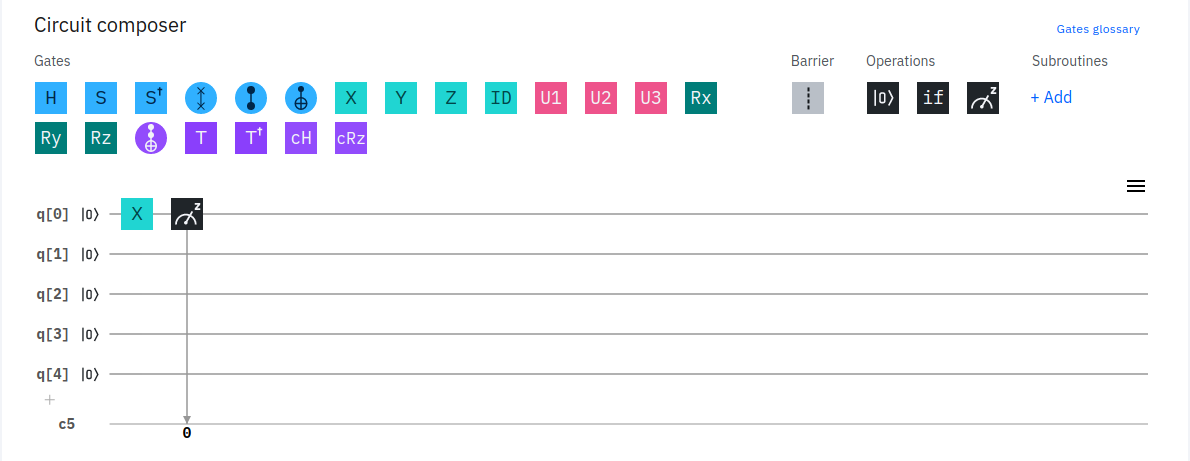
\includegraphics[width=1\textwidth]{figures/ibm_qx_composer.png} 
	\caption{Nástroj na tvorbu kvantových obvodov v IBM Quatnum Experience.}
    \label{ibm_qx_composer}
\end{figure}

Obvody je možné navrhovať aj pomocou špeciálneho jazyka OpenQASM, pomocou
editora, ktroý IBM QX obsahuje. Pri zobrazovaní výsledkov sa stav systému 
označuje pomocou klasických bitov. Teda pri navrhovaní programu pomocou
OpenQASM, je nutné definovať jednak počet kvantových a súčasne aj počet 
klasických bitov v systéme.

\begin{code}
qreg q[5];
creg c[5];
\end{code}

Je nutné podotknúť, že kvantový bit \(\psi_0\) je v IBM QX reprezentovaný
ako \(q[0]\), \(psi_1 = q[1]\) a tak ďalej. Pri meraní sa tieto bity zobrazia
do príslušných c registrov:
\begin{itemize}
\item[] \(q[0] \rightarrow c[0]\)
\item[] \(q[1] \rightarrow c[1]\)
\item[] \(\dots\)
\end{itemize}

Po inicializácií potrebných registrov je možné pristúpiť k definovaniu 
samotného obvodu. Pre dosiahnutie obvodu ako na obrázku \ref{ibm_qx_composer}
vyvoláme aplikáciu hradla \(X\) na bite \(q[0]\) a následne využijeme meranie.

\begin{code}
x q[5];
measure q[0] -> c[0];
\end{code}

\begin{figure} 
	\centering 
	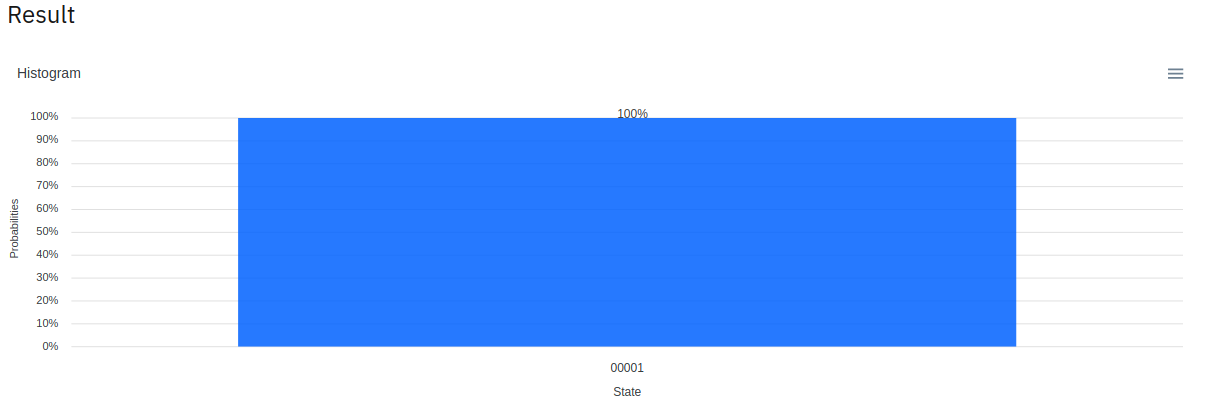
\includegraphics[width=1\textwidth]{figures/ibm_qx_results.png} 
	\caption{Výsledky exprimentu z IBM Quantum Experience.}
    \label{ibm_qx_results}
\end{figure}

Výsledky experimentov sa zobrazujú v stĺpcovom diagrame. Pričom stav systému
je zobrazovaný v klasických bitoch opačne ako v kvantových. Teda stav 
n-bitového systému \(\psi = \Ket{\psi_0\psi_1\psi_2 \dots \psi_{n-1}}\) je
meraný do klasického registra ako 
\[c_{n-1} \dots c_2 c_1 c_0\]
V našom prípade je
\[q[0] = X \Ket{0} =
\begin{pmatrix}
0 & 1\\
1 & 0\\
\end{pmatrix}
\binom{1}{0} = \binom{0}{1}
\]
, čo je \(1\) s pravdepodobnosťou \(1\). Teda výsledok na obrázku 
\ref{ibm_qx_results} zobrazuje, že kvantový systém dosiahne so \(100\%\) 
pravdepodobnosťou stav \(00001\).

\subsection{Stavy a ich zápis}

Pri výpočtoch je najviac využívaných týchto šesť stavov kvantových bitov:
\begin{itemize}
\item[] \(\Ket{0} = \binom{1}{0}\)
\item[] \(\Ket{1} = \binom{0}{1}\)
\item[] \(\Ket{+} = \frac{\Ket{0} + \Ket{1}}{\sqrt{2}}\)
\item[] \(\Ket{-} = \frac{\Ket{0} - \Ket{1}}{\sqrt{2}}\)
\item[] \(\Ket{\circlearrowright} = \frac{\Ket{0} - i\Ket{1}}{\sqrt{2}}\)
\item[] \(\Ket{\circlearrowleft} = \frac{\Ket{0} - i\Ket{1}}{\sqrt{2}}\)
\end{itemize}

Zmena stavu kvantového bitu je možná pomocou hradiel. Existuje viacero
hradiel, ktoré možno používať v kvantových systémoch. Aplikovaním hardiel
na rôznych stavoch dosiahneme rôznu zmenu. Prehľad aplikácií základných 
hradiel je v tabuľke \ref{hradla_vysl}.

\begin{table}
\begin{tabular}{|c|c||c|c|c|c|c|c|}
\hline
 & & \(\Ket{0}\) & \(\Ket{1}\) & \(\Ket{+}\) & \(\Ket{-}\) & \(\Ket{\circlearrowright}\) & \(\Ket{\circlearrowleft}\) \\
\hline
 & & \(\binom{1}{0}\) & \(\binom{0}{1}\) & \(\frac{1}{\sqrt{2}} \binom{1}{1}\) & \(\frac{1}{\sqrt{2}} \binom{1}{-1}\) & \(\frac{1}{\sqrt{2}}\binom{1}{i}\) & \(\frac{1}{\sqrt{2}} \binom{1}{-i}\) \\
\hline

\(X\) &  \(\begin{pmatrix}
0 & 1\\
1 & 0\\
\end{pmatrix} \) & \(\binom{0}{1}\) & \(\binom{1}{0}\) & \(\frac{1}{\sqrt{2}} \binom{1}{1}\) & \(\frac{1}{\sqrt{2}} \binom{-1}{1}\) & \(\frac{1}{\sqrt{2}} \binom{i}{1}\) & \(\frac{1}{\sqrt{2}} \binom{-i}{1}\) \\
\hline

\(Y\)  &  \(\begin{pmatrix}
0 & -i\\
i & 0\\
\end{pmatrix} \) & \(\binom{0}{i}\) & \(\binom{-i}{0}\) & \(\frac{1}{\sqrt{2}} \binom{-i}{i}\) & \(\frac{1}{\sqrt{2}} \binom{i}{i}\) & \(\frac{1}{\sqrt{2}} \binom{1}{i}\) & \(\frac{1}{\sqrt{2}} \binom{-1}{i}\) \\
\hline

\(Z\)  &  \(\begin{pmatrix}
1 & 0\\
0 & -1\\
\end{pmatrix} \) & \(\binom{1}{0}\) & \(\binom{0}{-1}\) & \(\frac{1}{\sqrt{2}} \binom{1}{-1}\) & \(\frac{1}{\sqrt{2}} \binom{1}{1}\) & \(\frac{1}{\sqrt{2}} \binom{1}{-i}\) & \(\frac{1}{\sqrt{2}} \binom{1}{i}\) \\
\hline

\(H\)  &  \(\frac{1}{\sqrt{2}}\begin{pmatrix}
1 & 1\\
1 & -1\\
\end{pmatrix} \) & \(\frac{1}{\sqrt{2}}\binom{1}{1}\) & \(\frac{1}{\sqrt{2}}\binom{1}{-1}\) & \(\binom{1}{0}\) & \(\binom{0}{1}\) & \(\frac{1}{\sqrt{2}} \binom{\frac{1+i}{\sqrt{2}}}{\frac{1-i}{\sqrt{2}}}\) & \(\frac{1}{\sqrt{2}} \binom{\frac{1-i}{\sqrt{2}}}{\frac{1+i}{\sqrt{2}}}\) \\
\hline

\(S\)  &  \(\begin{pmatrix}
1 & 0\\
0 & i\\
\end{pmatrix} \) & \(\binom{1}{0}\) & \(\binom{0}{i}\) & \(\frac{1}{\sqrt{2}} \binom{1}{i}\) & \(\frac{1}{\sqrt{2}} \binom{1}{-i}\) & \(\frac{1}{\sqrt{2}} \binom{1}{-1}\) & \(\frac{1}{\sqrt{2}} \binom{1}{1}\) \\
\hline

\(S^{\dag}\)  &  \(\begin{pmatrix}
1 & 0\\
0 & -i\\
\end{pmatrix} \) & \(\binom{1}{0}\) & \(\binom{0}{-i}\) & \(\frac{1}{\sqrt{2}} \binom{1}{-i}\) & \(\frac{1}{\sqrt{2}} \binom{1}{i}\) & \(\frac{1}{\sqrt{2}} \binom{1}{1}\) & \(\frac{1}{\sqrt{2}} \binom{1}{-1}\) \\
\hline

\(T\)  &  \(\begin{pmatrix}
1 & 0\\
0 & \frac{1+i}{\sqrt{2}}\\
\end{pmatrix} \) & \(\binom{1}{0}\) & \(\binom{0}{\frac{1+i}{\sqrt{2}}}\) & \(\frac{1}{\sqrt{2}} \binom{1}{\frac{1+i}{\sqrt{2}}}\) & \(\frac{1}{\sqrt{2}} \binom{1}{\frac{-1-i}{\sqrt{2}}}\) & \(\frac{1}{\sqrt{2}} \binom{1}{\frac{-1+i}{\sqrt{2}}}\) & \(\frac{1}{\sqrt{2}} \binom{1}{\frac{1-i}{\sqrt{2}}}\) \\
\hline

\(T^{\dag}\)  &  \(\begin{pmatrix}
1 & 0\\
0 & \frac{1-i}{\sqrt{2}}\\
\end{pmatrix} \) & \(\binom{1}{0}\) & \(\binom{0}{\frac{1-i}{\sqrt{2}}}\) & \(\frac{1}{\sqrt{2}} \binom{1}{\frac{1-i}{\sqrt{2}}}\) & \(\frac{1}{\sqrt{2}} \binom{1}{\frac{-1+i}{\sqrt{2}}}\) & \(\frac{1}{\sqrt{2}} \binom{1}{\frac{1+i}{\sqrt{2}}}\) & \(\frac{1}{\sqrt{2}} \binom{1}{\frac{-1-i}{\sqrt{2}}}\) \\
\hline
\end{tabular}

\caption{\label{hradla_vysl} Tabuľka stavov kvantových bitov a výsledky 
aplikácií hradiel na tieto stavy.}
\end{table}

%\subsection{Operacie kvantovych hradiel}
